\chapter{Udbredte racer i Kalish}
I dette kapitel bliver racerne i Kalish beskrevet. Da A’kastin er et af de centrale riger i Kalish, er alle racer repræsenteret her, på godt og ondt. Det betragtes som almen viden at kende til de forskellige racer. Vi anbefaler, at man tilpasser sit kostume til sin race, så det giver den bedste effekt i spillet. Samtidig anbefales det, at en karakters baggrundshistorien tilpasses det område, man kommer fra. Ved enkelte racer vil der være reelle krav, som skal opfyldes, inden man kan spille racen.\\
Husk på, at det er muligt at ansøge om at spille en anden race end dem, der står beskrevet her i hæftet. Faun, varulv, halvelver er blot tre eksempler på racer, der kan ansøges om.\\

\section{Menneske}
\begin{race*}[Mennesker]
\textbf{LP:} 2\\ 
\textbf{NK:} 2\\ 
\textbf{Evne:} Bære person\\
\textbf{Krav:} Ingen Makshøjde. Ingen kostumekrav\\
\rule{\textwidth}{0.4pt}
\textbf{Bære person:} Du kan nu bære andre personer. Dette kræver fysisk kontakt til personen, samt mere NK end denne, såfremt personen modsætter sig. Benyttelse af denne evne synliggøres ved at sige "bær person", når du ønsker en person skal følge med.\\
\end{race*}

Mennesker er, som du kender dem fra middelalderen, og er en god begynder race.\\
Fælles for alle mennesker er, at de er et arbejdende folk og ved, hvordan man tager fat. Ikke mindst når de skal hjælpe med at bygge barrikader, for at beskytte sig mod Kalishs mange fare. I A’kastins spilverden stammer mennesker fra tre egne i Kalish, og der, ud fra dit valg, giver din karakter forskellige evner, samt information omkring dit hjemland. 

\textbf{Mennesker fra Nordland}\\
\textit{Imperiet har hovedsæde i Nordland. Imperiet er det kejserige, som næsten alle mennesker er en del af. Her lever mennesker under stor disciplin fra Kejseren og hans veltrænede legionærhær, eller som robuste øksesvingende Nordlinge fra gletscheren.}\\
\textbf{Evner:} Mennesker fra Nordland kan altid bruge tohåndsvåben og har evnen Førstehjælp.\\
\textbf{Førstehjælp:} Du er i stand til at forbinde sårende i kamp vha. bandager (hvide bånd). Dette tager 30 sekunder.\\

\textbf{Mennesker fra Permersland}\\
\textit{Siden Dæmonkrigen har der været borgerkrig i Permersland med få fredspauser. Krigen splitter Nordland og Sydland, fordi Nordland ikke kunne betale sin gæld til Sydland. Mennesker i Permersland er hårdføre og kampvante. De lever splittet mellem hertugdømmerne eller lever som lejesvende.}\\
\textbf{Evne:} Mennesker fra Permersland får +2 NK.\\

\textbf{Mennesker fra Sydland}\\
\textit{Handelskompagniet ligger i Sydland. Her lever mennesker pompøst under stor velstand. Sydlands ressourcerige områder har medført, at selv den fattigste tigger altid kan finde klingende mønt.}\\
\textbf{Evne:} Mennesker fra Sydland får +5 Fjend ved hver spilgang, og har evnen Læse og Skrive.\\
\textbf{Læse og Skrive:} Du kan læse og skrive skrift, der er skrevet på det almindelige skriftsprog.\\




\section{Dværge}
\begin{race*}[Dværge]
\textbf{LP:} 3\\ 
\textbf{NK:} 4\\ 
\textbf{Evne:} Minearbejder\\
\textbf{Krav:} Makshøjde: 170 cm. Skæg, må godt være kunstigt. Kvindelige dværge behøver ikke skæg, men må gerne.\\
\rule{\textwidth}{0.4pt}
\textbf{Minearbejder:} Alle kan arbejde i minen, men med denne evne har du en chance for at finde ressourcer i stedet for ingenting eller Fjend.
\end{race*}

Dværgene stammer fra Livet Ende, som er et rige, hvor bjerge og frost hersker. Dværgene lever dybt inde i bjergene, beskyttet af deres store fæstninger. De er specialister i at udøve deres håndværk, som strækker sig lige fra smedning til ølbrygning. Dværge respekterer ikke magi, men bruger i stedet runernes kraft eller gudernes velsignelser. Da grænserne til Livets Ende er lukket, eksisterer der ikke mange dværge i de andre dele af Kalish.\\
Dværgene lever i forskellige krak. Dette er kæmpestore byer som befinder sig under vulkaner. Hver klan har deres eget krak.\\


\textbf{Dværge fra Hammerens krak}\\
\textit{Dværgene fra Hammerens krak er lærde og håndværkere. De opfinder, bygger og smeder med alt, de kan få fingrene i. De kan komme fra Livets Ende eller Antikvariatet, som er den store bankboks med magiske genstande i Nordland.}\\
\textbf{Evner:} Reparere rustning Niv. 1 og Lave låse Niv. 1\\
\textbf{Reparere rustning Niv. 1:} Du kan genoprette 1 RP på ødelagt rustning, når du benytter 2 min på at reparere denne. Dette kan gentages indtil rustningen fremstår 'uden skader'.\\
\textbf{Lave låse Niv. 1:} Du kan nu lave låse i Niv. 1. Disse låse kan påsættes på både punge, tasker og kister, for at beskytte dem fra uvedkommende. Nedenfor ses en beskrivelse af hvad det kræver at fremstille en lås. Dette kræver 2 jern og 15 minutters arbejde med hammer og armbolt.\\


\textbf{Dværge fra Øksens krak}\\
\textit{Du skal aldrig beskytte dine knæskaller, medmindre du møder en dværg fra Øksens Krak. De er opvokset med at hamre Sortelvere i de uendelige kampe, der finder sted i dybet under Livets Ende. Kamp, disciplin og vildskab flyder i disse dværgeårer.}\\
\textbf{Evner:} Dværge fra dette krak får +1 LP og +1 NK.

\section{Halvlang}
\begin{race*}[Halvlange]
\textbf{LP:} 1\\ 
\textbf{NK:} 1\\ 
\textbf{Evne:} Bonk, 6. sans Niv. 1 \& Lommetyveri Niv. 1\\
\textbf{Krav:} Makshøjde: 170 cm. Ingen kostumekrav.\\
\rule{\textwidth}{0.4pt}
\textbf{Bonk:} Du kan 'bonke' andre personer. Dette gøres ved at ligge et våben på en anden persons skulder, hvorefter der tydeligt skal siges "Bonk!".\\
Herefter vil personen falde om og besvime, men ikke miste LP. Denne person vil forblive besvimet i 10 min eller indtil personen tager skade eller bliver vækket af en anden person. Den besvimmede person kan gennemsøges og vil glemme de sidste 10 min inden personen blev 'bonket'.\\
\textbf{6. Sans Niv. 1:} Du er immun over for lommetyveri Niv. 1.\\
\textbf{Lommetyveri Niv. 1:} Med Lommetyveri Niv. 1 kan du lægge din hånd på offerets pung i 15 sekunder, for derefter at stjæle alt (undtagen de sidste 3 mønter) i pungen. Offeret ved ikke, at de er blevet bestjålet.\\
\end{race*}

Halvlange stammer oprindeligt fra Livets Ende, men nu om dage kan de findes overalt i Kalish. En halvlang er et lille, muntert væsen, som meget sjældent bliver sur og vred. Hvis man opsøger dem, kan man næsten altid være sikker på at møde en venlig person, som hellere ville byde dig på et krus øl og en god historie end et slagsmål. Som halvlang kan du få selv den kedeligste samtale til at blomstre og berige dine lommer.

\section{Elver}
\begin{race*}[Elvere]
\textbf{LP:} 3\\ 
\textbf{NK:} 2\\ 
\textbf{Evne:} Læse og skrive Elvisk.\\
\textbf{Krav:} Der er ingen makshøjde. Man skal have spidse ører.\\
\rule{\textwidth}{0.4pt}
\textbf{Læse og skrive Elvisk:} Du kan læse og skrive skrift, der er skrevet på Elvisk.\\
\end{race*}

\begin{figure}[H]
    \centering
    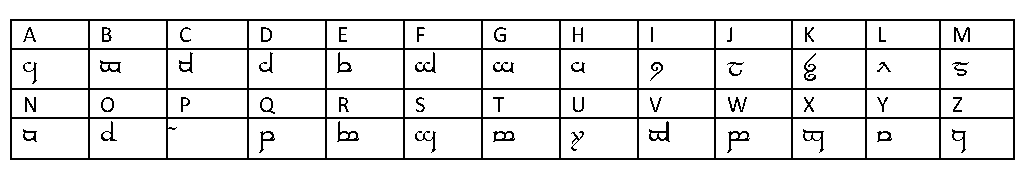
\includegraphics[width=1\textwidth]{../Evne-Ordbog/setup/Alfabeter/Elvisk alfabet.pdf}
    \caption{Elvisk alfabet}
\end{figure}

Elverne fødes fra træernes skyggeside eller dybets mørke, når Måne og Sol mødes i foråret. Det er altid en stor begivenhed, når en elver skabes. De synges med langvarige, magiske remser ud af et gammelt træ eller træernes rødder, i de magiske skove omkring Mek, af den grund sætter de stor pris på deres liv og føler sig hævet over Kalishs andre racer.\\
De magiske omstændigheder for deres skabelse medfører, at deres antal er begrænset; og endnu mere efter Dæmonkrigen, hvor de fleste af elverne døde i forsøget på at beskytte de underlegne racer fra dæmonernes hærgen.\\

\textbf{Højelvere}\\
\textit{Højelverne er beskytterne af Azken Kanpe og magi. De kan stadig finde barmhjertighed overfor de underlegne racer. De bruger de livsskabende energier i Kalish til at være til stede, observere og for at hindre fremtidens Dæmonkrige.}\\
\textbf{Evne:} Hvis en Højelver kan kaste magi, tæller de som at have +2 maksimal mana. Hvis en Højelver ikke kan kaste magi tæller de som at have 2 mana, der genvindes hver time.\\

\textbf{Skovelver}\\
\textit{I skovene omkring Azken Kanpe og ud til Meks grænser lever Skovelverne. De mindes altid de faldne fra Dæmonkrigen, og lever efter at skyde først og spørge bagefter, når det handler om at beskytte Mek. Det rygtes, at Skovelverne kan se de hvileløse ånder, og kan bringe dem til hvile i træerne.}\\
\textbf{Evne:} Som skov elver får man +1 NK og Påfør gift.\\
\textbf{Påfør gift:} Du kan påføre gifte som vil give skade på et våben. Våbnet skal have et blad, så som
kniv, sværd eller ligende, og må ikke være et projektil, så som pile eller en kastet kastekniv. Giften vil kun vare på det næste slag eller til våbnet gives til en anden person,
hvor efter giften vil forsvinde.\\
Når et våben bruges på denne måde skal ordene: "Gift kniv x i skade"siges. Her vil x være hvor meget skade du giver med giften. Skulle giften have andre effekter end skade skal disse ikke siges da de ignoreres.\\


\textbf{Sortelver}\\
\textit{I det dybeste mørke under Livets Ende lever Sortelverne. Deres kvinder har altid det sidste ord. I mellemtiden står alle mændene til på et tidspunkt at tjene i de uendelige kampe mod dværgene. Efter deres gud Daikia døde under gudekrigene har hendes Datter Ishtar taget magten. Alle Daikia's børn er kendt som Ilsherne. Sortelver samfundet er delt op i Huse, repræsenteret med en farve. Ishtars hus er det hvide hus. Sortelvere er sky, arrogante og værdsætter smerte og død.}\\
\textbf{Evne:} Du får evnen Påfør gift og Rygte Spreder/Samler Niv. 1\\
\textbf{Påfør gift:} Du kan påføre gifte som vil give skade på et våben. Våbnet skal have et blad, så som
kniv, sværd eller ligende, og må ikke være et projektil, så som pile eller en kastet kastekniv. Giften vil kun vare på det næste slag eller til våbnet gives til en anden person,
hvor efter giften vil forsvinde.\\
Når et våben bruges på denne måde skal ordene: "Gift kniv x i skade"siges. Her vil x være hvor meget skade du giver med giften. Skulle giften have andre effekter end skade skal disse ikke siges da de ignoreres.\\
\textbf{Rygte Spreder/Samler Niv. 1}
Du kan stille et spørgsmål til en arrangør om, hvad der sker i Akastin eller starte et rygte blandt spillerne.\\
\textbf{Krav:} Som sortelver skal du males sort på alle synlige steder.\\


\section{Grønhuder}
Grønhuderne findes i næsten hele Kalish, men er mest udbredt i de uendelig sletter. Orker er en gåde for de fleste mennesker. Det ene øjeblik kan de virke som harmløse væsner, og det næste kan de gå amok og vil tæske dig med dine egne arme.\\
Ingen ved med sikkerhed hvordan orkerne blev til, eller hvordan de fødes. Nogle orker mener, de faldt ned fra himlen, da der var en stor kamp i gang. Nogle akademikere mener at orkerne er en form for svampeorganismer, der er vokset op af dyngerne af restaffald, som grønhudsgrupperne efterlader.\\
En enlig grønhud bliver set som let bytte af de andre racer, og derfor færdes de sjældent alene. Grønhuder lever for én ting, hvilket er kamp og jagt. De søger altid at jage den største trussel inden for deres leveområde. Det er ikke unormalt, at en grønhud “BOSS” bliver skiftet ud.\\
Grønhuderne viser aldrig frygt - det vil sige, ikke med vilje. Deres primitive levemåde gør dem brutale, og man skal tænke sig godt om, inden man lægger sig ud med dem. For dem er jagten ALT!.
\begin{race*}[Gobliner]
\textit{Goblinen er den mindste grønhud. De holder altid sammen, og ved, hvad der skal til for at overleve, for mange hjerner gør dig klog. Derfor er det oftest goblinerne, der tænker for grønhuderne; men det er stadig bossen, som bestemmer.}\\
\\
\textbf{LP:} 1\\ 
\textbf{NK:} 1\\ 
\textbf{Evne:} Lommetyveri Niv. 1\\
\textbf{Krav:} Makshøjde: 170 cm. Som goblin skal du være malet en lys grøn på alle synlige steder.\\
\rule{\textwidth}{0.4pt}\\
\textbf{Lommetyveri Niv. 1:} Med Lommetyveri Niv. 1 kan du lægge din hånd på offerets pung i 15 sekunder, for derefter at stjæle alt (undtagen de sidste 3 mønter) i pungen. Offeret ved ikke, at de er blevet bestjålet.\\
\end{race*}

\begin{race*}[Ork]
\textit{Orken er grim, stærk og snotdum. De lever for at slås, og for at tage livet af alt, der ikke er med i grønhudstammen.}\\
\\
\textbf{LP:} 3\\ 
\textbf{NK:} 4\\ 
\textbf{Evne:} Bære person\\
\textbf{Krav:} Minimumshøjde: 170 cm. Som ork skal du være malet mørk grøn på alle synlige steder.\\
\textbf{Restriktioner:} Orken snakker meget dårligt menneskesprog, og kender sjældent de rigtige ord for ting.\\
\rule{\textwidth}{0.4pt}\\
\textbf{Bære person:} Du kan nu bære andre personer. Dette kræver fysisk kontakt til personen, samt mere NK end denne, såfremt personen modsætter sig. Benyttelse af denne evne synliggøres ved at sige "bær person", når du ønsker en person skal følge med.\\
\end{race*}

\begin{race*}[Blodork - Kræver specialansøgning]
\textit{Blodorken bliver ikke skabt som de andre grønhuder. Denne form for ork nærmer sig grænsen til det monstrøse. De er større og mere brutale end normale orker, og er resultatet af Hrothgars korruption af orkerne under dæmonernes hærgen. De første blodorker blev til under dæmonkrigene i landet A’kastin, da verden flød med dæmoner og orkerne ikke havde andet føde end dæmonsteg, og ikke havde andet vand end blodet fra dem. Dette gjorde, at de efterhånden udviklede sig til større og mere aggressive orker; blodorker. Blodorkerne er fjendtlige og aggressive, og stort set umulige at nedkæmpe ene mand.}\\
\\
\textbf{LP:} 6\\ 
\textbf{NK:} 6\\ 
\textbf{Evne:} Krigsleder\\
\textbf{Krav:} Minimumshøjde: 170 cm. Som blodork skal du være malet mørk/sort grøn på alle synlige steder.\\
\textbf{Restriktioner:} En Blodork kan ikke snakke med andre end grønhuder. De skal bruge en goblin eller en ork til at oversætte for sig. (Dette er blandt andet for inkludere yngre spillere i voksen spil, dette er derfor et blødt krav som kan ignoreres hvis der ikke er nogen gobliner eller orkere omkring dig.).\\
\rule{\textwidth}{0.4pt}\\
\textbf{Krigsleder:} Når en goblin ser en blodork vil goblinens kampgejst blive forøget. Gobliner som kan se en blodork vil få 1 LP og + 1 NK. LP’et er det første der mistes i kamp og kan ikke genvindes før næste slag.\\
\textbf{Vigtigt!} En goblin kan kun få denne effekt af en blodork. Hvis orkhæren har 3 blodorker vil goblinerne i hæren kun modtage 1 ekstra LP og ikke 3.\\
\end{race*}

\begin{race*}[Trold - Kræver specialansøgning]
\textit{Trolden er alle grønhudernes hemmelige våben. Disse kæmper er utrolig dovne og dumme. I kamp vågner de dog, og trolden er en brutal og nådesløs, der knuser alt på sin vej. Ingen døre eller porte kan holde den tilbage, og trolden kan alene kæmpe sig igennem disse.}\\
\\
\textbf{LP:} 10\\ 
\textbf{NK:} 10\\ 
\textbf{Evne:} Udvidet Naturlig Helbredelse\\
\textbf{Krav:} Minimumshøjde: 180 cm. Som Trold skal du være malet mørk grålig grøn på alle synlige steder.\\
\textbf{Restriktioner:} En Trold kan ikke snakke med andet end grønhuder. De skal bruge en goblin eller en ork til at oversætte for sig. (Dette er blandt andet for inkludere yngre spillere i voksen spil).\\
\rule{\textwidth}{0.4pt}\\
\textbf{Udvidet Naturlig Helbredelse:} Din naturlige helbredelse vil blive forbedret, så du nu vil genvinde 1 LP pr. 5 min.\\
\end{race*}